\section{Experiments}

Testdata has been generated by a python script that, given a $N$,
generates a \verb|FASTA| file with two sequenses on length $N$. The
two algorithms, affine and linear, was then run 10 times on input
size, and the running time averaged. The timing was done with the unix
tool \verb|perf|.

The machine that ran the tests has the following specs:
\begin{description}
\item[CPU:] Intel i7 quadcore 2.67GHz
\item[RAM:] 6GB
\item[Operating System:] Ubuntu 14.04 LTS
\item[Python version:] 3.4.0
\end{description}

This first plot shows $N$ on the horizontal axis and the actual
(average) running time divided by the expected asymptotic complexity
($O(N^2)$) on the vertical axis. The plot shows that sub-quadratic
factors play an overwhelming role on datasets smaller than $N \approx
100$.
\begin{center}
	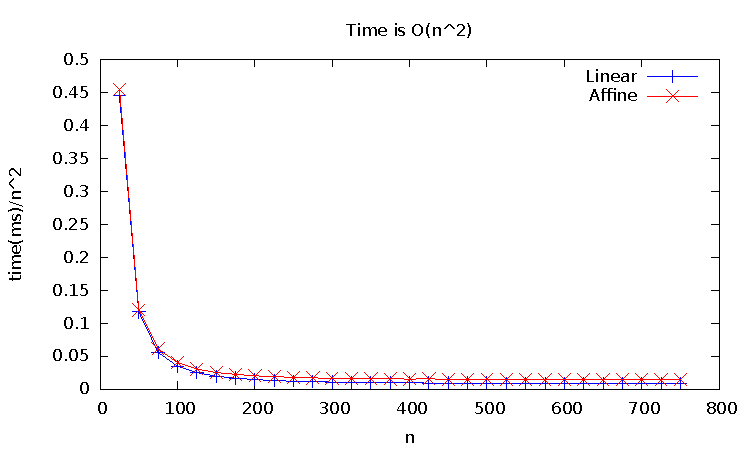
\includegraphics[width=\textwidth]{../plots/plot1.pdf}
\end{center}

In this second plot, we have zoomed in on roughly the lower half of
the plot from before. Both lines seem to approach horizontal as $N$
increases. This suggests that the asymptotic complexity of $O(N^2)$ is
right.
\begin{center}
	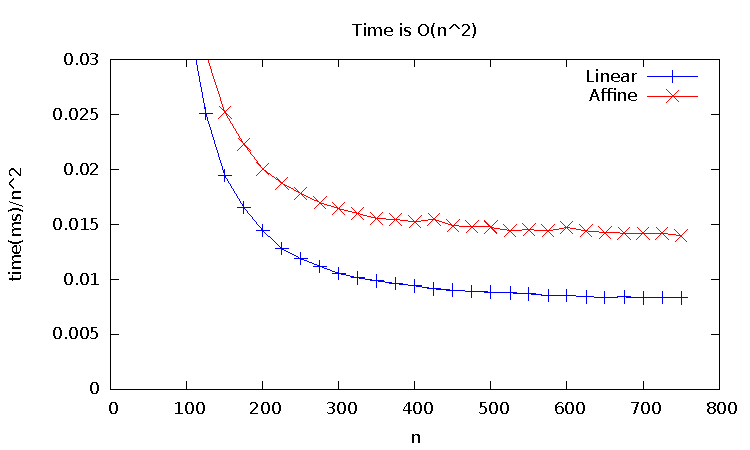
\includegraphics[width=\textwidth]{../plots/plot2.pdf}
\end{center}

The last plot shows the ratio between the execution times of the two
algorithms. It can be seen that they are roughly equally fast in the
beginning, but as $N$ increases towards 400, the linear algorithm
becomes comparatively faster than the affine algorithm. Around $N
\approx 400$ it seems to stabilize as $T(affine)/T(linear) \approx
1.7$, meaning that the affine algorithm takes approximately 70\%
longer than the corresponding linear case.
\begin{center}
	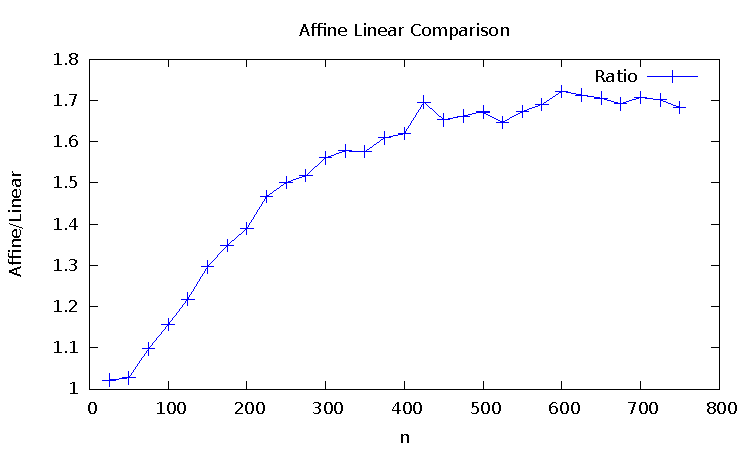
\includegraphics[width=\textwidth]{../plots/plot3.pdf}
\end{center}
